\documentclass{beamer}

\usetheme{CambridgeUS}
\usecolortheme{dolphin}

\usepackage{wrapfig}
\usepackage{siunitx}
%\usepackage{inconsolata}
\usepackage{amsmath}
\usepackage{bm}
\usepackage{adjustbox}
\usepackage{nicefrac}
\usepackage{namelist}

%\usepackage[backend=bibtex,style=authoryear]{biblatex}
%\bibliography{common/references}
%\AtBeginBibliography{\scriptsize}

% Tikz
\usepackage{tikz}
\usetikzlibrary{positioning,shapes,arrows,calc,intersections}
\usepackage{pgfplots}
\usepgfplotslibrary{dateplot}
\pgfplotsset{compat=1.8}

\DeclareMathOperator{\spann}{span}
\DeclareMathOperator{\tr}{tr}

\definecolor{darkblue}{HTML}{00688B}
\definecolor{darkgreen}{HTML}{6E8B3D}
\definecolor{cadet}{HTML}{DAE1FF}
\definecolor{salmon}{HTML}{FFB08A}

\setbeamercovered{transparent}
\setbeamercolor{alerted text}{fg=red}

\AtBeginSection[]{
  \begin{frame}
  \vfill
  \centering
  \begin{beamercolorbox}[sep=8pt,center,shadow=true,rounded=true]{title}
    \usebeamerfont{title}\insertsectionhead\par%
  \end{beamercolorbox}
  \vfill
  \end{frame}
}

\begin{document}

\title[Poroelastic fracturing]{
  Poroelastic fracturing
}
\author[T.~Kvamsdal]{
  T.~Kvamsdal\inst{1,2} \and
  E.~Fonn\inst{2} \and
  A.~M.~Kvarving\inst{2} \and
  K.~M.~Okstad\inst{2} \and
  K.~Johannessen\inst{2} \and
}
\institute[NTNU/SINTEF]{
  \and \inst{1}%
  Department of Mathematical Sciences, NTNU
  \and \inst{2}%
  Applied Mathematics and Cybernetics, SINTEF Digital
}
\date[Nov 2019]{}

\titlegraphic{
  \includegraphics[height=0.05\textheight]{common/ntnu} \hspace{0.1\textheight}
  \includegraphics[height=0.05\textheight]{common/sintef}
}

\newcommand<>{\malert}[1]{{\color#2{red}#1}}

\begin{frame}
  \titlepage
\end{frame}

\section{Physical model}

\begin{frame}
  \frametitle{Poroelasticity}

  \begin{itemize}
  \item Fundamental conservation of momentum
    \[
      \nabla \cdot \malert<2>{\bm \sigma^\text{t}} + \malert<3>{\rho} \malert<4>{\bm f_\text{b}} = \bm 0
    \]
  \item<5-> Darcy flow: contribution to stress
    \[
      \bm \sigma^\text{t} = \malert<6>{\bm \sigma^\text{e}} + \malert<7>{\alpha} \malert<8>{p} \bm I
    \]
  \item<9-> Darcy flow: mass balance equation
    \[
      \alpha \nabla \cdot \malert<10>{\dot{\bm u}} + \malert<11-12>{\frac{1}{M}} \dot{p} - \nabla \cdot
      \left[ \malert<13>{\bm \kappa} \cdot (\nabla p - \malert<14>{\rho_\text{f}} \bm f_\text{b}) \right] = \malert<15>{q_\text{b}}
    \]
  \end{itemize}

  \begin{overlayarea}{\textwidth}{1cm}
    \begin{center}
      \color{red}{
        \only<2>{$\bm \sigma^\text{t}$: total stress}%
        \only<3>{$\rho$: total mass density}%
        \only<4>{$\bm f_\text{b}$: body forces}%
        \only<6>{$\bm \sigma^\text{e} = \bm \sigma(\bm \varepsilon)$: effective stress}%
        \only<7>{$\alpha$: Biot's coefficient (typically $\alpha = 1$)}%
        \only<8>{$p$: pressure of fluid in porous material --- a primary unknown}%
        \only<10>{$\bm u$: displacement vector field --- a primary unknown}%
        \only<11>{$\nicefrac{1}{M}$: specific storage coefficient, a measure of compressibility of fluid}%
        \only<12>{\vspace{-1cm}\[\frac{1}{M} = \frac{\alpha - n}{K_\text{s}} + \frac{n}{K_\text{f}}\]}%
        \only<13>{$\bm \kappa$: permeability tensor field}%
        \only<14>{$\rho_\text{f}$: fluid density}%
        \only<15>{$q_\text{b}$: fluid sources and sinks}%
      }
    \end{center}
  \end{overlayarea}
\end{frame}

\begin{frame}
  \frametitle{Poroelasticity}

  System of equations resulting from variational formulation
  \begin{align*}
    \bm u_i, \delta \bm u_i &\in H^1(\Omega)^d \\
    p_i, \delta p_i &\in \left\{ p \in L^2(\Omega) \;\Big|\; \int_\Omega p = 0 \right\}
  \end{align*}
  \[
    \begin{pmatrix} & \\ \malert<2>{\bm Q^\intercal} & \malert<3>{\bm S} \end{pmatrix}
    \begin{pmatrix} \dot{\bm u} \\ \dot{\bm p} \end{pmatrix} +
    \begin{pmatrix} \malert<5>{\bm K} & \malert<2>{- \bm Q} \\ & \malert<4>{\bm P} \end{pmatrix}
    \begin{pmatrix} \bm u \\ \bm p \end{pmatrix} =
    \begin{pmatrix} \malert<6>{\bm f_u} \\ \malert<7>{\bm f_p} \end{pmatrix}
  \]

  \begin{overlayarea}{\textwidth}{1cm}
    \begin{center}
      \color{red}{
        \only<2>{The coupling matrix \[ \bm Q_{ij} = \alpha \int_\Omega \nabla \delta \bm u_j : p_i \bm I \]}%
        \only<3>{The storativity matrix \[ \bm S_{ij} = \int_\Omega c \delta p_i p_j \]}%
        \only<4>{The permeability matrix \[ \bm P_{ij} = \int_\Omega \nabla \delta p_i^\intercal \bm \kappa \nabla p_j \]}%
        \only<5>{The stiffness matrix
          \[ \bm K_{ij} = \int_\Omega \bm \varepsilon(\delta \bm u_i) : \bm D \bm \varepsilon(\bm u_j) \]}%
        \only<6>{Momentum load
          \[ (\bm f_u)_i = \int_\Omega \delta \bm u_i \cdot \rho \bm f_\text{b}
            + \int_{\Gamma_\text{n}} \delta \bm u_i \cdot \overline{\bm t} \]}%
        \only<7>{Flux load \[ (\bm f_p)_i = \int_\Omega \delta \bm p_i q_\text{b} \] }%
      }
    \end{center}
  \end{overlayarea}
\end{frame}

\begin{frame}
  \frametitle{Poroelasticity}

  \begin{itemize}
  \item Note that $\bm K$ and $\bm f_u$ are ``standard'' elasticity
    system matrices
  \item<2-> This serves as a convenient ``plugging point'' for
    substituting different elasticity models in the same Darcy flow
    interpretation
  \item<3-> E.g. dynamic elasticity
    \[
      \begin{pmatrix} \malert<4>{\bm M} & \\ & \end{pmatrix}
      \begin{pmatrix} \ddot{\bm u} \\ \ddot{\bm p} \end{pmatrix} +
      \begin{pmatrix} \malert<5>{\bm C} & \\ \bm Q^\intercal & \bm S \end{pmatrix}
      \begin{pmatrix} \dot{\bm u} \\ \dot{\bm p} \end{pmatrix} +
      \begin{pmatrix} \bm K & - \bm Q \\ & \bm P \end{pmatrix}
      \begin{pmatrix} \bm u \\ \bm p \end{pmatrix} =
      \begin{pmatrix} \bm f_u \\ \bm f_p \end{pmatrix}
    \]
  \end{itemize}

  \begin{overlayarea}{\textwidth}{1cm}
    \begin{center}
      \color{red}{
        \only<4>{The mass matrix \[ M_{ij} = \int_\Omega \delta \bm u_i \cdot \bm u_j \]}%
        \only<5>{The damping matrix \[ \bm C = a \bm M + b \bm K \]}%
      }
    \end{center}
  \end{overlayarea}
\end{frame}

\begin{frame}
 \frametitle{Domain with internal discontinuity}

 \begin{center}
   \includegraphics[trim=0cm 0cm 20cm 0cm, clip=true, width=0.6\textwidth]{figs/crack}
 \end{center}
\end{frame}

\begin{frame}
  \frametitle{Energy functional for dynamic brittle fracture}

  \[
    \Psi(\bm{u},\dot{\bm{u}},\Gamma) = \int_\Omega\left(
      \frac{\rho}{2}\dot{\bm{u}}\cdot\dot{\bm{u}} - \psi_e(\bm{u}) \right) -
    \int_\Gamma {\cal G}_c
  \]
  where
  %
  \begin{namelist}{Gc}
  \item[$\Gamma$] is the unknown crack path
  \item[$\psi_e$] = $\frac{1}{2}\lambda(\tr \bm \varepsilon)^2 +
    \mu\tr(\bm{\varepsilon}:\bm{\varepsilon})$
    ~is the strain energy density function, \\
    $\lambda$ and $\mu$ are the Lam\`e material parameters, \\ and
    $\bm{\varepsilon}(\bm{u})$ is the 2nd-order strain tensor
  \item[${\cal G}_c$] is the fracture energy density
  \end{namelist}
\end{frame}

\begin{frame}
  \frametitle{Phase-field approximation of the discontinuity}

  \begin{center}
    \includegraphics[trim=16cm 0cm 0cm 0cm, clip=true, width=0.7\textwidth]{figs/crack}
  \end{center}
\end{frame}

\begin{frame}
  \frametitle{Phase-field model}

  \begin{itemize}
  \item Resolves individual cracks down to some length scale
  \item Diffuse interface $\Rightarrow$ no interface tracking
  \end{itemize}

  \begin{columns}[c]
    \column{0.45\textwidth}
    \includegraphics[width=0.9\textwidth]{figs/phasefield}
    \column{0.55\textwidth}
    \[
      \left\{
        \begin{array}{lcl}
          c = 1     &\Rightarrow& \mbox{undamaged material} \\
          0 < c < 1 &\Rightarrow& \mbox{damaged material} \\
          c = 0     &\Rightarrow& \mbox{cracked material}
        \end{array}
      \right.
    \]
  \end{columns}
\end{frame}

\begin{frame}
  \frametitle{Energy functional for dynamic brittle fracture}

  \begin{itemize}
  \item Approximation of the fracture energy:
    \[
      \int_\Gamma {\cal G}_c \approx
      \left\{
        \begin{array}{ll}
          \int_\Omega {\cal G}_c\left(
          \frac{(1-c)^2}{4\ell_0} + \ell_0|\nabla c|^2 \right) & \mbox{2nd-order} \\
          \int_\Omega {\cal G}_c\left(
          \frac{(1-c)^2}{4\ell_0} + \frac{\ell_0}{2}|\nabla c|^2
          + \frac{\ell_0^3}{4}(\nabla^2c)^2 \right) & \mbox{4th-order}
        \end{array}
      \right.
    \]
    where $c\in[0,1]$ is the phase field parameter,
    and $\ell_0$ is a chosen length scale defining the ``thickness''
    of the damaged material (crack) zone.
  \item Split of elastic strain energy density into tensile and compressive parts
    \[
      \psi_e(\bm{u}) = g(c)\psi^+(\bm{\varepsilon}) + \psi^-(\bm{\varepsilon})
    \]
    where $g(c)$ is a degradation function (typically chosen as $c^2$), and
    $\psi^+$ and $\psi^-$ are tensile and compressive contributions, respectively
  \end{itemize}
\end{frame}

\begin{frame}
  \frametitle{Small strain brittle fracture}

  \begin{itemize}
  \item Strain tensor:
    \[
      \bm{\varepsilon}(\bm{u}) = \frac{1}{2}\left(\nabla\bm{u} + (\nabla\bm{u})^T\right)
    \]
  \item Stress tensor:
    \[
      \bm{\sigma}(\bm{u}) =
      \frac{\partial}{\partial\bm{\varepsilon}}\psi_e(\bm{\varepsilon}) =
      g(c)\frac{\partial}{\partial\bm{\varepsilon}}\psi^+(\bm{\varepsilon}) +
      \frac{\partial}{\partial\bm{\varepsilon}}\psi^-(\bm{\varepsilon})
    \]
  \item Minimizing
    $\Psi(\bm{u},\dot{\bm{u}},\Gamma)\approx\Psi(\bm{u},\dot{\bm{u}},c)$
    with respect to $\bm{u}$ and $c$ yields the strong form of the
    brittle crack problem:
    \begin{align*}
      \nabla\cdot\bm{\sigma}(\bm{u}) &= \rho\ddot{\bm{u}} & \text{linear momentum} \\
      \frac{2\ell_0}{{\cal G}_c}g'(c)\psi^+ + c - 4\ell_0^2\nabla^2c &= 1 & \text{phase-field (2nd-order)} \\
      \frac{2\ell_0}{{\cal G}_c}g'(c)\psi^+ + c - 2\ell_0^2\nabla^2c + \ell_0^4\nabla^4c &= 1 & \text{Phase-field (4th-order)}
    \end{align*}
    on $\Omega\times]0,T]$.
  \end{itemize}
\end{frame}

\begin{frame}
  \frametitle{Strain history field}

  To ensure that the developed crack does not close again, i.e.,
  $\Gamma(t)\subset\Gamma(t+\Delta t) ~~\forall~\Delta t > 0$, the tensile energy
  density $\psi^+$ in the phase-field equation is replaced by a history field
  ${\cal H}(\bm{x},t)$, satisfying ${\cal H}\ge\psi^+$, $\dot{\cal H}\ge0$ and
  $\dot{\cal H}({\cal H} - \psi^+) = 0$.
  Thus
  \begin{align*}
    \frac{2\ell_0}{{\cal G}_c}g'(c){\cal H} + c - 4\ell_0^2\nabla^2c &= 1 & \text{(2nd-order)} \\
    \frac{2\ell_0}{{\cal G}_c}g'(c){\cal H} + c - 2\ell_0^2\nabla^2c + \ell_0^4\nabla^4c &= 1 & \text{(4th-order)}
  \end{align*}
\end{frame}

\begin{frame}
  \frametitle{Boundary and initial conditions}
  \[
    \begin{array}{rclcll}
      u_\alpha &=& g_\alpha &\mbox{on}& \partial\Omega_{g_\alpha}\times[0,T] & \mbox{: Dirichlet condition on~} u_\alpha \\
      \sigma_{\alpha\beta}n_\beta &=& h_\alpha &\mbox{on}& \partial\Omega_{h_\alpha}\times[0,T] & \mbox{: Neumann condition on the} \\ & & & & &
                                                                                                                                                 ~~\alpha \mbox{th traction component} \\
      \nabla c\cdot\bm{n} &=& 0 &\mbox{on}& \Omega\times[0,T] & \mbox{: Neumann condition on~} c
    \end{array}
  \]
  \[
    \begin{array}{rclcll}
      \bm{u}(\bm{x},0) &=& \bm{u}_0(\bm{x}) &\forall& \bm{x}\in\Omega &
                                                                        \mbox{: Initial condition on displacement} \\
      \dot{\bm{u}}(\bm{x},0) &=& \bm{v}_0(\bm{x}) &\forall& \bm{x}\in\Omega &
                                                                              \mbox{: Initial condition on velocity} \\
      {\cal H}(\bm{x},0) &=& {\cal H}_0(\bm{x}) &\forall& \bm{x}\in\Omega &
                                                                            \mbox{: Initial strain-history field}
    \end{array}
  \]
  A non-zero ${\cal H}_0$ can be used to model pre-existing cracks or other
  geometric features to be captured by the mesh topology, e.g.
  \[
    {\cal H}_0(\bm{x}) =
    \left(\frac{1}{c_0}-1\right)\frac{{\cal G}_c}{4\ell_0}
    \left(1-\min\left\{\frac{d(\bm{x},l)}{\ell_0},1\right\}\right)
  \]
  where $d(\bm{x},l)$ denotes the shortest distance from $\bm{x}$ to the curve $l$
  describing the initial crack geometry, and $c_0$ is phase-field value in the
  initial crack.
\end{frame}

\begin{frame}
  \frametitle{Spectral decomposision of strains}

  To establish the tensile ($\psi^+$) and compressive ($\psi^-$) contributions
  of the elastic strain energy, the eigenvalues, $\lambda_\alpha$, and associated
  egenvectors, $\bm{n}_\alpha$, of the strain tensor $\bm{\varepsilon}$,
  are computed such that
  \begin{align*}
    \bm{\varepsilon} &=
    \sum_\alpha\lambda_\alpha\,\bm{n}_\alpha\otimes\bm{n}_\alpha =
    \malert<3>{\bm{\varepsilon}^+} + \malert<4>{\bm{\varepsilon}^-} \\
    &= \malert<3>{\sum_\alpha\malert<2>{\langle\lambda_\alpha\rangle}\,\bm{n}_\alpha\otimes\bm{n}_\alpha} +
    \malert<4>{\sum_\alpha(\lambda_\alpha-\malert<2>{\langle\lambda_\alpha\rangle})\,\bm{n}_\alpha\otimes\bm{n}_\alpha}
  \end{align*}
  \onslide<5->{
    Then
    \begin{align*}
      \psi^+ &= \frac{\lambda}{2}\langle\tr\bm{\varepsilon}\rangle^2 +
               \mu\tr(\bm{\varepsilon}^+:\bm{\varepsilon}^+) \\
      \psi^- &= \frac{\lambda}{2}(\tr\bm{\varepsilon}-\langle\tr\bm{\varepsilon}\rangle)^2 +
               \mu\tr(\bm{\varepsilon}^-:\bm{\varepsilon}^-)
    \end{align*}
  }
  \begin{overlayarea}{\textwidth}{1cm}
    \begin{center}
      \color{red}{
        \only<2>{$\langle x \rangle = \nicefrac{1}{2}(x + |x|)$, the positive part of $x$}%
        \only<3>{$\bm \varepsilon^+$: the tensile strain tensor}%
        \only<4>{$\bm \varepsilon^-$: the compressive strain tensor}%
      }
    \end{center}
  \end{overlayarea}
\end{frame}

% \begin{frame}
%   \frametitle{Fracturing}
%   \begin{center}
%     \includegraphics[trim=0cm 0cm 20cm 0cm, clip=true, width=0.7\textwidth]{figs/crack}
%   \end{center}
% \end{frame}

% \begin{frame}
%   \frametitle{Fracturing}

%   \begin{itemize}
%   \item<1-> Represent material damage in terms of an \emph{integrity field} $c : \Omega \to [0,1]$
%     \begin{itemize}
%     \item $c = 1 \Longrightarrow$ undamaged material (high integrity)
%     \item $c = 0 \Longrightarrow$ fully destroyed material (no integrity)
%     \end{itemize}
%   \item<2-> The evolution of $c$ is governed by the Cahn-Hilliard equation
%     \[
%       \malert<3>{\eta} \dot{c} + \malert<5>{(c - \malert<6>{\ell}^2 \Delta c)} = - c \malert<4>{\mathcal{H}}
%     \]
%   \item<7-> $\mathcal{H}(t)$ is a quantity derived from the current
%     tensile stress. In practice, irreversibility must be enforced, e.g.
%     \[
%       \mathcal{H}(t_n) = \max \left\{ \mathcal{H}(t_{n-1}), \Psi(\bm \sigma(t_n)) \right\}
%     \]
%   \end{itemize}

%   \begin{overlayarea}{\textwidth}{1cm}
%     \begin{center}
%       \color{red}{
%         \only<3>{$\eta$: a material parameter}%
%         \only<4>{$\mathcal{H}$: the \emph{crack driving force}}%
%         \only<5>{geometric resistance term (second order)}%
%         \only<6>{$\ell$: regularization length scale}%
%       }
%     \end{center}
%   \end{overlayarea}
% \end{frame}

% \begin{frame}
%   \frametitle{Fracturing}
%   \begin{center}
%     \includegraphics[trim=16cm 0cm 0cm 0cm, clip=true, width=0.8\textwidth]{figs/crack}
%   \end{center}
% \end{frame}

% \begin{frame}
%   \frametitle{Fracturing}

%   \begin{itemize}
%   \item The effect of $c$ on the elasticity model is realized by
%     ``diluting'' the tensile elastic energy, e.g. by writing
%     \[
%       \bm \sigma^\text{e} = \malert<4>{g(c)} \malert<2>{\bm \sigma^{(+)}} + \malert<3>{\bm \sigma^{(-)}}
%     \]
%   \item<5-> This has the effect of non-linearizing the elasticity
%     model, even if it were already linear
%   \end{itemize}

%   \begin{overlayarea}{\textwidth}{1cm}
%     \begin{center}
%       \color{red}{
%         \only<2>{$\bm \sigma^{(+)}$: tensile stress (positive principal components of $\bm \sigma^\text{e}$)}%
%         \only<3>{$\bm \sigma^{(-)}$: compressive stress (negative principal components of $\bm \sigma^\text{e}$)}%
%         \only<4>{$g(c)$: relaxation factor, e.g. $g(c) = (1-k)c^2 + k$ for some $0 < k \ll 1$}%
%       }
%     \end{center}
%   \end{overlayarea}
% \end{frame}

\begin{frame}
  \frametitle{Flow in fractures}

  \vspace{-1cm}
  \begin{center}
    \includegraphics[width=0.6\textwidth]{figs/flux}
  \end{center}
  \vspace{-5mm}

  \begin{itemize}
  \item The effect of $c$ on the Darcy flow is realized by
    artificially inflating permeability in open fractures, to model
    Poiseuille flow.
    \[
      \bm \kappa_\text{m} = \malert<6>{\kappa} \bm I + (1-c)^b \left(
        \frac{w^2}{12} - \malert<6>{\kappa}
      \right) (\bm I - \malert<3>{\bm n \bm n^\intercal})
    \]
  \item<2-> $w$ is the regularized crack width, $w^2 = (\malert<4>{\lambda_\perp} - 1)^2 \malert<5>{L_\perp^2} \chi_{c<c_\text{crit}}$
  \end{itemize}

  \begin{overlayarea}{\textwidth}{1cm}
    \begin{center}
      \color{red}{
        \only<3>{The crack normal vector in physical coordinates
          \[
            \bm n = \frac{(\nabla \bm u)^{-\intercal} \nabla c}{|(\nabla \bm u)^{-\intercal} \nabla c|}
          \]
        }%
        \only<4>{The local perpendicular stretch
          \[
            \lambda_{\perp} = (\nabla \bm u) \frac{\nabla c}{|\nabla c|} \cdot \bm n
          \]
        }%
        \only<5>{$L_\perp$: length scale roughly tracing $\ell$ and meshwidth}%
        \only<6>{$\kappa$: isotropic un-fractured permeability}%
      }
    \end{center}
  \end{overlayarea}
\end{frame}

\section{Coupling and nonlinearities}

\begin{frame}
  \frametitle{Superiterations}

  \begin{itemize}
  \item Two primary solvers
    \begin{description}
    \item[A] Joint poroelastic solver for displacement and pressure
    \item[B] Separate solver for integrity
    \end{description}
  \item<2-> Solution for each timestep obtained in an interlaced manner
    (standard coupling technique)
    \begin{enumerate}
      \item solve A for $(\bm u_{n+1}^{(1)}, p_{n+1}^{(1)})$
      \item solve B for $c_{n+1}^{(1)}$
      \item solve A for $(\bm u_{n+1}^{(2)}, p_{n+1}^{(2)})$
      \item solve B for $c_{n+1}^{(2)}$
      \item etc.
    \end{enumerate}
  \item<3-> Fully coupled all-in-one solvers for all three unknowns have also been successful
  \end{itemize}
\end{frame}

\begin{frame}
  \frametitle{Subiterations}

  \begin{itemize}
  \item The poroelastic solver A must itself also be iterative
  \item<2-> Multiple sources of nonlinearity:
    \begin{itemize}
    \item due to the tensile/compressive energy splitting
    \item due to inherently nonlinear elasticity models
    \item due to iterative time solvers for dynamic problems (e.g. Newmark)
    \end{itemize}
  \end{itemize}

  \onslide<3->{
    Backward Euler for quasistatic problems
    \[
      \begin{pmatrix}
        \malert{\bm K(c)} & - \bm Q \\ \bm Q^\intercal / \delta_t & \malert{\bm P(c)} + \bm S / \delta_t
      \end{pmatrix}
      \begin{pmatrix}
        \bm u \\ \bm p
      \end{pmatrix}_{n+1} =
      \begin{pmatrix}
        \bm f_u \\ \bm f_p
      \end{pmatrix}_{n+1} +
      \begin{pmatrix}
        & \\ \bm Q^\intercal & \bm S
      \end{pmatrix}
      \begin{pmatrix}
        \bm u \\ \bm p
      \end{pmatrix}_{n+1}
    \]
  }
\end{frame}

\begin{frame}
  \frametitle{Newmark for dynamic problems}

  Given
  $\malert<2>{\bm a_{n+1}^i} = (\ddot{\bm u}, \ddot{\bm p})_{n+1}^i$,
  $\malert<2>{\bm v_{n+1}^i} = (\dot{\bm u}, \dot{\bm p})_{n+1}^i$,
  $\malert<2>{\bm d_{n+1}^i} = (\bm u, \bm p)_{n+1}^i$

  \onslide<3->{
    Solve
    \begin{align*}
      \malert<7>{\bm M^*} \Delta \bm a =
      \begin{pmatrix} \bm f_u \\ \bm f_p \end{pmatrix}_{n+1}
      - \malert<4>{\tilde{\bm M}} \bm a_{n+1}^i
      - \malert<5>{\tilde{\bm C}} \bm v_{n+1}^i
      - \malert<6>{\tilde{\bm K}} \bm d_{n+1}^i
    \end{align*}
  }

  \onslide<8->{
    \vspace{-5mm} Correct
    \begin{align*}
      \bm a_{n+1}^{i+1} &= \bm a_{n+1}^i + \Delta \bm a \\
      \bm v_{n+1}^{i+1} &= \bm v_{n+1}^i + \malert<9>{\gamma} \delta_t \Delta \bm a \\
      \bm d_{n+1}^{i+1} &= \bm d_{n+1}^i + \malert<9>{\beta} \delta_t^2 \Delta \bm a
    \end{align*}
  }

  \begin{overlayarea}{\textwidth}{1cm}
    \begin{center}
      \vspace{-5mm}
      \color{red}{
        \only<2>{\emph{Predicted} values for acceleration, velocity and solution}%
        \only<4>{$\tilde{\bm M} = \begin{pmatrix} \bm M & \\ & \end{pmatrix}$}%
        \only<5>{$\tilde{\bm C} = \begin{pmatrix} \bm C & \\ \bm Q^\intercal & \bm S \end{pmatrix}$}%
        \only<6>{$\tilde{\bm K} = \begin{pmatrix} \bm K & - \bm Q \\ & \bm P \end{pmatrix}$}%
        \only<7>{$\bm M^* = \tilde{\bm M} + \gamma \delta_t \tilde{\bm C} + \beta \delta_t^2 \tilde{\bm K}$}%
        \only<9>{Stability: $2\beta \ge \gamma \ge \nicefrac{1}{2}$, accuracy: $\gamma = \nicefrac{1}{2}$ }%
      }
    \end{center}
  \end{overlayarea}
\end{frame}

\begin{frame}
  \frametitle{Adaptivity}

  \begin{itemize}
  \item Adaptive refinement is almost mandatory
    \begin{itemize}
    \item Fractures require high spatial resolution to resolve well (see: $\ell$)
    \item \ldots but only locally
    \end{itemize}
  \item<2-> Refining elements with small $c$ \alert{\emph{a posteriori}} is
    dubious: fractures propagate slower through coarse meshes
  \item<3-> Thus a third layer of iterations: whenever refinement is
    needed, re-run the last handful of timesteps on the finer mesh.
  \end{itemize}
\end{frame}

\section{Adaptive mesh refinement of the crack path}

\begin{frame}
  \frametitle{Adaptive mesh refinement}

  \begin{itemize}
  \item A fine mesh resolution is required to correctly capture the crack development.
  \item Using a fine uniform mesh is easiest and safest, but too costly.
  \item An adaptive strategy that refines the mesh only where the crack is propagating is needed.
  \item We use a multi-pass procedure, using the phase-field value as refinement criterium.
  \item A linear or quadratic LR B-Spline discretization is used,
    allowing for local refinement.
  \item When an initial crack is present, the mesh is refined based on the
    distance $d^{c0}_e$ from the element center to the initial crack path,
    before the simulation is started.
  \end{itemize}
\end{frame}

\begin{frame}
  \frametitle{Adaptive mesh refinement, initial state}

  \begin{tabbing} XXX\=X\=\kill
    $\bullet$ Load the initial, uniform, background mesh \\[2mm]
    $\bullet$ $d^\text{tol}$ \>\> = min. distance to initial crack path for non-refined elements \+\+\\
    $\approx h^0$ (characteristic element size of the initial mesh) \-\-\\[2mm]
    ~~FOR $i = 1$ TO number of initial refinement cycles DO \+\\[1mm]
    $\bullet$  Refine all elements $e$, where $d^{c0}_e < d^\text{tol}$ \\
    $\bullet$ $d^\text{tol} = d^\text{tol} / 2$ \-\\[1mm]
    ~~END DO
  \end{tabbing}
\end{frame}

\begin{frame}
  \frametitle{Adaptive mesh refinement, multi-pass algorithm}

  % 1      2        3      4
  \begin{tabbing} X\=XX\=X\=X\=X\=X\=XX\=X\=\kill
    $\bullet$ \> $n_\text{step}$ \>\>\> = total number of time steps \\
    $\bullet$ \> $n_\text{step}^c$ \>\>\> = number of time steps in each refinement cycle \\
    $\bullet$ \> $n_\text{cycle}$ \>\>\> = max. number of refinement cycles before continuing \+\\[2mm] %1
    FOR $i = 1$ TO $n_\text{step}$ DO ! Time step loop \+\+\\[2mm] %2
    FOR $j = 1$ TO $n_\text{cycle}$ TO \+\+\\[1mm]
    $\bullet$ \> Restore solution state for time $t_{i-1}$ \+\\ %3
    FOR $k = 0$ TO $n_\text{step}^c-1$ TO \+\\ %4
    $\bullet$ \> Compute elasticity and phase-field solutions at time $t_{i+k}$ \-\\ %3
    END DO \-\\
    $\bullet$ \> Refine all elements $e$, for which $|c|_e < c_\text{tol}$ \+\\
    IF no elements were refined THEN exit DO-loop \-\-\-\\ %2
    END DO \-\\ %1
    $\bullet$ \> $i = i + n_\text{step}^c$ \-\\
    END DO
  \end{tabbing}
\end{frame}

\section{Pre-notched Rectangular Plate}

\begin{frame}
  \frametitle{Pre-notched rectangular plate}

  \begin{columns}[c]
    \column{0.7\textwidth}
    \includegraphics[width=\textwidth]{figs/Rectangle}
    \column{0.3\textwidth}
    \begin{align*}
      \rho &= \SI{2450}{\kilo\gram/\meter^3} \\
      E &= \SI{32}{\giga\pascal} \\
      \nu &= 0.2 \\
      {\cal G}_c &= \SI{3}{\joule/\meter}
    \end{align*}
  \end{columns}
\end{frame}

\begin{frame}
  \frametitle{Mesh and time step size}

  \begin{center}
    \begin{tabular}{c|ccrc}
      Mesh & $p$ & $n_\text{el}$ & $n_\text{dof}$~ & $\delta_t$ [s] \\\hline
      % U1   &  1  &  129122 & ~$1.0\times10^-7$ \\
      % U2   &  1  &  514242 & ~$5.0\times10^-8$ \\
      % U3   &  1  & 2052482 & ~$2.5\times10^-8$ \\\hline
      U1   &  2  & ~$400\times160$ &  133650 & ~$1.0\times10^{-7}$ \\
      U2   &  2  & ~$800\times320$ &  523250 & ~$5.0\times10^{-8}$ \\
      U3   &  2  & $1600\times640$ & 2066580 & ~$2.5\times10^{-8}$ \\\hline
      A0   &  2  & 4054 &  7676 & ~$1.0\times10^{-7}$ \\
      $\vdots$ &  & $\vdots$ & $\vdots$~~~ & \\
      A$n$ &  2  & 8686 & 15648 & ~$1.0\times10^{-7}$
      % A1   &  1  &    7488 & $4.95\times10^-7$ \\
      % A2   &  1  &   17440 & ~$2.5\times10^-7$ \\
      % A3   &  1  &   41268 & ~$1.0\times10^-7$ \\
      % A4   &  1  &   96282 & ~$1.0\times10^-7$ \\\hline
      % A1   &  2  &    7760 & $4.95\times10^-7$ \\
      % A2   &  2  &   18768 & ~$2.5\times10^-7$ \\\hline
    \end{tabular}
  \end{center}
\end{frame}

\begin{frame}
  \frametitle{Elastic energy}
  \begin{center}
    \includegraphics[width=0.8\textwidth]{figs/elasticEnergy-p2} \\
    \begin{picture}(0,0)
      \put(-70,70){$ \varepsilon_e = \int_\Omega\left(c^2\psi^+ + \psi^-\right) $}
    \end{picture}
  \end{center}
\end{frame}

\begin{frame}
  \frametitle{Elastic energy, uniform meshes}
  \begin{center}
    \includegraphics[width=0.8\textwidth]{figs/elasticEnergy-UMR} \\
    \begin{picture}(0,0)
      \put(-70,70){$ \varepsilon_e = \int_\Omega\left(c^2\psi^+ + \psi^-\right) $}
    \end{picture}
  \end{center}
\end{frame}

\begin{frame}
  \frametitle{Elastic energy, adapted meshes}
  \begin{center}
    \includegraphics[width=0.8\textwidth]{figs/elasticEnergy-AMR}
  \end{center}
\end{frame}

\begin{frame}
  \frametitle{Dissipated energy}
  \begin{center}
    \includegraphics[width=0.8\textwidth]{figs/dissipEnergy-p2} \\
    \begin{picture}(0,0)
      \put(-90,180){$ \varepsilon_d = \int\limits_\Omega{\cal
          G}_c\left[\frac{(c-1)^2}{4\ell_0} + \ell_0(\nabla
          c)^2\right]dV $}
    \end{picture}
  \end{center}
\end{frame}

\begin{frame}
  \frametitle{Dissipated energy, uniform meshes}
  \begin{center}
    \includegraphics[width=0.8\textwidth]{figs/dissipEnergy-UMR} \\
    \begin{picture}(0,0)
      \put(-90,180){$ \varepsilon_d = \int\limits_\Omega{\cal
          G}_c\left[\frac{(c-1)^2}{4\ell_0} + \ell_0(\nabla
          c)^2\right]dV $}
    \end{picture}
  \end{center}
\end{frame}

\begin{frame}
  \frametitle{Dissipated energy, adapted meshes}
  \begin{center}
    \includegraphics[width=0.8\textwidth]{figs/dissipEnergy-AMR}
  \end{center}
\end{frame}

\begin{frame}
  \frametitle{Phase-field for Mesh U1, p=2}
  \begin{overlayarea}{\textwidth}{0.7\textheight}
    \begin{center}
      \only<1>{%
        \includegraphics[width=0.9\textwidth]{figs/Borden-U1-p2} \\[5mm]
        from M.\ J.\ Borden {\it et al}.,
        ``A phase-field description of dynamic brittle fracture'',
        Comput.\ Methods Appl.\ Mech.\ Engrg. 217--220 (2012) 77--95.
      }%
      \only<2>{%
        \includegraphics[width=\textwidth]{figs/Rectangle-U1-p2-2nd} \\[5mm]
        with IFEM
      }%
      \only<3>{%
        \includegraphics[width=\textwidth]{figs/Rectangle-U1-p2-4th} \\[5mm]
        with IFEM (4th order phase field)
      }%
    \end{center}
  \end{overlayarea}
\end{frame}

\begin{frame}
  \frametitle{Phase-field for Mesh U2, p=2}
  \begin{overlayarea}{\textwidth}{0.7\textheight}
    \begin{center}
      \only<1>{%
        \includegraphics[width=0.9\textwidth]{figs/Borden-U2-p2} \\[5mm]
        from M.\ J.\ Borden {\it et al}.,
        ``A phase-field description of dynamic brittle fracture'',
        Comput.\ Methods Appl.\ Mech.\ Engrg. 217--220 (2012) 77--95.
      }%
      \only<2>{%
        \includegraphics[width=\textwidth]{figs/Rectangle-U2-p2-2nd} \\[5mm]
        with IFEM
      }%
    \end{center}
  \end{overlayarea}
\end{frame}

\def\pfline#1#2{
  \put(#1,142){\hskip-10pt\scriptsize$#2$}
  \put(#1,0){\color{red}\line(0,1){140}}
}

\begin{frame}
  \frametitle{Phase-field on adapted mesh, p=2}

  \begin{center}
    \includegraphics[width=0.897\textwidth]{figs/Rectangle-p2-adap3-c02}\newline
    \begin{picture}(0,0)
      % \pfline{16}{x=0}
      % \pfline{307}{x=100}
      \pause\pfline{30.6}{x=60}
      \pause\pfline{59.7}{x=70}
      \pause\pfline{88.8}{x=80}
      \pause\pfline{117.9}{x=90}
    \end{picture}
  \end{center}
\end{frame}

\begin{frame}
  \frametitle{Phase-field on 4th adapted mesh, p=1}

  \begin{center}
    \includegraphics[width=\textwidth]{figs/Rectangle-A4-p1}
  \end{center}
\end{frame}

%%%%%%%%%%%%%%%%%%%%%%%%%%%%%%%%%%%%%%%%%%%%%%%%%%%%%%%%%%%%%%%%%%%%%%%%%%%%%%%%

\begin{frame}
  \only<1>{\frametitle{Phase field along the vertical line $x=60$ at $t=\SI{0.079}{\milli\second}$}}
  \only<2>{\frametitle{Phase field along the vertical line $x=70$ at $t=\SI{0.079}{\milli\second}$}}
  \only<3>{\frametitle{Phase field along the vertical line $x=80$ at $t=\SI{0.079}{\milli\second}$}}
  \only<4>{\frametitle{Phase field along the vertical line $x=90$ at $t=\SI{0.079}{\milli\second}$}}

  \begin{center}
    \only<1>{%
      \includegraphics[width=0.8\textwidth]{figs/Line-x60}%
    }%
    \only<2>{%
      \includegraphics[width=0.8\textwidth]{figs/Line-x70}%
    }%
    \only<3>{%
      \includegraphics[width=0.8\textwidth]{figs/Line-x80}%
    }%
    \only<4>{%
      \includegraphics[width=0.8\textwidth]{figs/Line-x90}%
    }%
  \end{center}
\end{frame}

\section{Pre-notched square plate}

\begin{frame}
  \frametitle{Pre-notched square plate}

  \begin{columns}[c]
    \column{0.6\textwidth}
    \includegraphics[width=0.9\textwidth]{figs/SquareWithNotch}
    \column{0.4\textwidth}
    \begin{align*}
      E &= \SI{210}{\kilo\newton/\milli\meter^2} \\
      \nu &= 0.3 \\
      {\cal G}_c &= \SI{2.7}{\milli\newton/\milli\meter} \\
      \ell_0 &= \SI{0.0075}{\milli\meter}
    \end{align*}
    Adaptive with 3, 4 and 5 refinement levels \\[2mm]
    $p=1,2$ (LR B-splines) \\[2mm]
    a) Tension test \\
    b) Pure shear test
  \end{columns}
  \vskip\baselineskip
  \scriptsize(Figure from C.\ Miehe, M.\ Hofacker, F.\ Welschinger,
  A phase field model for rate-independent crack propagation: Robust algorithmic
  implementation based on operator splits. Computer Methods in Applied Mechanics and Engineering,
  vol.\ 199 (2010), pp.\ 2765--2778.)
\end{frame}

\def\xline#1#2{%\pause (somehow the \pause did not work in this environment)
  \put(#1,18){\color{yellow}\line(0,1){24}}
  \put(#1,16.3){\hskip-5pt\scriptsize\color{yellow}#2}
}

\begin{frame}
  \frametitle{Tension test, initial crack by $C^{-1}$-continuity}

  \begin{center}
    \setlength{\unitlength}{1mm}
    \only<1>{
      \begin{picture}(60,60)
        \thicklines
        \put(0,0){\includegraphics[width=60mm]{testTension/Miehe51_C-1_slit-initial}}
        \put(0,0){\line(1,0){60}}
        \put(0,0){\line(0,1){60}}
        \put(0,60){\line(1,0){60}}
        \put(60,0){\line(0,1){60}}
        \put(0,30){\line(1,0){30}}
      \end{picture}
    }\only<2>{
      \begin{picture}(60,60)
        \thicklines
        \put(0,0){\includegraphics[width=60mm]{testTension/Miehe51_C-1_slit-final}}
        \put(0,0){\line(1,0){60}} \put(0,0){\line(0,1){60}}
        \put(0,60){\line(1,0){60}} \put(60,0){\line(0,1){60}}
        \put(0,30){\line(1,0){40.5}}
        \xline{30}{0.5}\put(22,16.3){\color{yellow}\scriptsize$x=$}
        \xline{36}{0.6}
        \xline{42}{0.7}
        \xline{48}{0.8}
        \xline{54}{0.9}
        \xline{60}{1.0}
      \end{picture}
    }
  \end{center}
\end{frame}

\begin{frame}
  \only<1>{\frametitle{Tension test, phase field along $x=0.5$ at $t=0.7$}}
  \only<2>{\frametitle{Tension test, phase field along $x=0.6$ at $t=0.7$}}
  \only<3>{\frametitle{Tension test, phase field along $x=0.7$ at $t=0.7$}}
  \only<4>{\frametitle{Tension test, phase field along $x=0.8$ at $t=0.7$}}
  \only<5>{\frametitle{Tension test, phase field along $x=0.9$ at $t=0.7$}}
  \only<6>{\frametitle{Tension test, phase field along $x=1.0$ at $t=0.7$}}

  \begin{center}
    \only<1>{%
      \includegraphics[width=\textwidth]{figs/islit-40x40-x05-t=07}%
    }%
    \only<2>{%
      \includegraphics[width=\textwidth]{figs/islit-40x40-x06-t=07}%
    }%
    \only<3>{%
      \includegraphics[width=\textwidth]{figs/islit-40x40-x07-t=07}%
    }%
    \only<4>{%
      \includegraphics[width=\textwidth]{figs/islit-40x40-x08-t=07}%
    }%
    \only<5>{%
      \includegraphics[width=\textwidth]{figs/islit-40x40-x09-t=07}%
    }%
    \only<6>{%
      \includegraphics[width=\textwidth]{figs/islit-40x40-x10-t=07}%
    }%
  \end{center}
\end{frame}

\begin{frame}
  \frametitle{Tension test, reaction force vs.~displacement}

  \begin{center}
    \includegraphics[width=\textwidth]{testTension/Staggered/Miehe51-slit}
  \end{center}
\end{frame}

\begin{frame}
  \frametitle{Tension test, initial crack by phase field}

  \begin{center}
    \setlength{\unitlength}{1mm}
    \only<1>{%
      \begin{picture}(60,60)
        \thicklines
        \put(0,0){\includegraphics[width=60mm]{testTension/Miehe51-initial}}
        \put(0,0){\line(1,0){60}}
        \put(0,0){\line(0,1){60}}
        \put(0,60){\line(1,0){60}}
        \put(60,0){\line(0,1){60}}
        \put(0,30){\line(1,0){30}}
      \end{picture}%
    }%
    \only<2>{%
      \begin{picture}(60,60)
        \thicklines
        \put(0,0){\includegraphics[width=60mm]{testTension/Miehe51-final}}
        \put(0,0){\line(1,0){60}} \put(0,0){\line(0,1){60}}
        \put(0,60){\line(1,0){60}} \put(60,0){\line(0,1){60}}
        \put(0,30){\line(1,0){40.5}}
        \xline{30}{0.5}\put(22,16.3){\color{yellow}\scriptsize$x=$}
        \xline{36}{0.6}
        \xline{42}{0.7}
        \xline{48}{0.8}
        \xline{54}{0.9}
        \xline{60}{1.0}
      \end{picture}%
    }%
  \end{center}
\end{frame}

\begin{frame}
  \only<1>{\frametitle{Tension test, phase field along $x=0.5$ at $t=0.63$}}
  \only<2>{\frametitle{Tension test, phase field along $x=0.6$ at $t=0.63$}}
  \only<3>{\frametitle{Tension test, phase field along $x=0.7$ at $t=0.63$}}
  \only<4>{\frametitle{Tension test, phase field along $x=0.8$ at $t=0.63$}}
  \only<5>{\frametitle{Tension test, phase field along $x=0.9$ at $t=0.63$}}
  \only<6>{\frametitle{Tension test, phase field along $x=1.0$ at $t=0.63$}}

  \begin{center}
    \only<1>{%
      \includegraphics[width=\textwidth]{figs/40x40-x05-t=063}%
    }%
    \only<2>{%
      \includegraphics[width=\textwidth]{figs/40x40-x06-t=063}%
    }%
    \only<3>{%
      \includegraphics[width=\textwidth]{figs/40x40-x07-t=063}%
    }%
    \only<4>{%
      \includegraphics[width=\textwidth]{figs/40x40-x08-t=063}%
    }%
    \only<5>{%
      \includegraphics[width=\textwidth]{figs/40x40-x09-t=063}%
    }%
    \only<6>{%
      \includegraphics[width=\textwidth]{figs/40x40-x10-t=063}%
    }%
  \end{center}
\end{frame}

\def\yline#1#2{%\pause (does not work)
  \put(18,#1){\color{yellow}\line(1,0){24}}
  \put(10.4,#1){\scriptsize\color{yellow}$#2$}
}

\begin{frame}
  \frametitle{Shear test, initial crack by $C^{-1}$-continuity}

  \begin{center}
    \setlength{\unitlength}{1mm}
    \only<1>{%
      \begin{picture}(60,60)
        \thicklines
        \put(0,0){\includegraphics[width=60mm]{testShear/Miehe52-initial.png}}
        \put(0,0){\line(1,0){60}}
        \put(0,0){\line(0,1){60}}
        \put(0,60){\line(1,0){60}}
        \put(60,0){\line(0,1){60}}
        \put(0,30){\line(1,0){30}}
      \end{picture}
    }%
    \only<2>{%
      \begin{picture}(60,60)
        \thicklines
        \put(0,0){\includegraphics[width=60mm]{testShear/Miehe52-final.png}}
        \put(0,0){\line(1,0){60}}
        \put(0,0){\line(0,1){60}}
        \put(0,60){\line(1,0){60}}
        \put(60,0){\line(0,1){60}}
        \put(0,30){\line(1,0){30}}
        \yline{30}{y=0.5}
        \yline{24}{y=0.4}
        \yline{18}{y=0.3}
        \yline{12}{y=0.2}
        \yline{6}{y=0.1}
      \end{picture}
    }%
  \end{center}
\end{frame}

\begin{frame}
  \only<1>{\frametitle{Shear test, phase field along $y=0.5$ at $t=2$}}
  \only<2>{\frametitle{Shear test, phase field along $y=0.4$ at $t=2$}}
  \only<3>{\frametitle{Shear test, phase field along $y=0.3$ at $t=2$}}
  \only<4>{\frametitle{Shear test, phase field along $y=0.2$ at $t=2$}}
  \only<5>{\frametitle{Shear test, phase field along $y=0.1$ at $t=2$}}

  \begin{center}
    \only<1>{%
      \includegraphics[width=\textwidth]{figs/40x40-y05-t=2}%
    }%
    \only<2>{%
      \includegraphics[width=\textwidth]{figs/40x40-y04-t=2}%
    }%
    \only<3>{%
      \includegraphics[width=\textwidth]{figs/40x40-y03-t=2}%
    }%
    \only<4>{%
      \includegraphics[width=\textwidth]{figs/40x40-y02-t=2}%
    }%
    \only<5>{%
      \includegraphics[width=\textwidth]{figs/40x40-y01-t=2}%
    }%
  \end{center}
\end{frame}

\begin{frame}
  \frametitle{Shear test, reaction force vs.~displacement}

  \begin{center}
    \includegraphics[width=\textwidth]{figs/Miehe52-forces}
  \end{center}
\end{frame}

\section{L-shaped domain}

\begin{frame}
  \frametitle{L-shaped domain}

  \begin{columns}[c]
    \column{0.6\textwidth}
    \includegraphics[width=0.9\textwidth]{figs/Lshape}
    \column{0.4\textwidth}
    \begin{align*}
      E &= \SI{25.85}{\mega\newton/\milli\meter^2} \\
      \nu &= 0.18 \\
      {\cal G}_c &= \SI{0.09}{\kilo\newton/\milli\meter} \\
      \ell_0 &= \SI{1.875}{\milli\meter}
    \end{align*}
    \small The displacement $u$ \\ is applied over a \\ $\SI{10}{\milli\meter}$ wide segment
  \end{columns}
  \vskip\baselineskip
  \footnotesize(Figure from M.\ Ambati, T.\ Gerasimov, L.\ De Lorenzis,
  A review on phase-field models of brittle fracture and a new fast hybrid formulation.
  Computational Mechanics, vol.\ 55 (2014), pp.\ 383--405.)
\end{frame}

\begin{frame}
  \frametitle{L-shaped domain, 5 patches, $3 \times 50 \times 50$, $p=1$}

  \begin{center}
    \setlength{\unitlength}{1mm}
    \begin{picture}(60,60)
      \thicklines
      \only<1>{\put(0,0){\includegraphics[width=60mm]{testLshape/Lshape-3x50x50-initial}}}
      \only<2>{\put(0,0){\includegraphics[width=60mm]{testLshape/Lshape-3x50x50-final}}}
      \put(0,0){\line(1,0){30}}
      \put(0,0){\line(0,1){60}}
      \put(0,30){\line(1,0){60}}
      \put(0,60){\line(1,0){60}}
      \put(30,0){\line(0,1){60}}
      \put(55.9,30){\line(0,1){30}}
      \put(57,30){\line(0,1){30}}
      \put(60,30){\line(0,1){30}}
      \thinlines
      \put(55.8,25.9){\vector(0,1){3.7}}
      \put(56.4,25.9){\vector(0,1){3.7}}
      \put(57,25.9){\vector(0,1){3.7}}
      \put(55.8,25.9){\line(1,0){1.2}}
      \put(55.3,23.4){$u$}
    \end{picture} \\
    \only<1>{Initial grid}
    \only<2>{Final grid}
  \end{center}
\end{frame}

\begin{frame}
  \frametitle{L-shaped domain, 5 patches, $3 \times 25 \times 25$, $p=1$}

  \begin{center}
    \setlength{\unitlength}{1mm}
    \begin{picture}(60,60)
      \thicklines
      \only<1>{\put(0,0){\includegraphics[width=60mm]{testLshape/Lshape-3x25x25-initial}}}
      \only<2>{\put(0,0){\includegraphics[width=60mm]{testLshape/Lshape-3x25x25-final}}}
      \put(0,0){\line(1,0){30}}
      \put(0,0){\line(0,1){60}}
      \put(0,30){\line(1,0){60}}
      \put(0,60){\line(1,0){60}}
      \put(30,0){\line(0,1){60}}
      \put(55.9,30){\line(0,1){30}}
      \put(57,30){\line(0,1){30}}
      \put(60,30){\line(0,1){30}}
      \thinlines
      \put(55.8,25.9){\vector(0,1){3.7}}
      \put(56.4,25.9){\vector(0,1){3.7}}
      \put(57,25.9){\vector(0,1){3.7}}
      \put(55.8,25.9){\line(1,0){1.2}}
      \put(55.3,23.4){$u$}
    \end{picture} \\
    \only<1>{Initial grid}
    \only<2>{Final grid}
  \end{center}
\end{frame}

\section{The Sneddon case}

\begin{frame}
  \frametitle{The Sneddon Case}

  \begin{itemize}
  \item Square domain with a pre-formed horizontal crack in the middle, with some prescribed
    half-length $\ell$.
  \item<2-> The crack is pressurized with a flux, causing widening and potentially crack propagation.
  \end{itemize}

  \begin{center}
    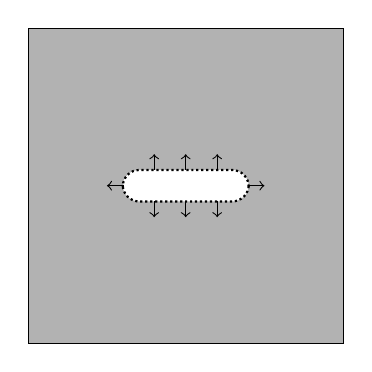
\begin{tikzpicture}[scale=2]
      \draw[fill=black!30] (-1,-1) rectangle (1,1);
      \draw[rounded corners=6, densely dotted, thick, fill=white] (-.4,-.1) rectangle (.4,.1);
      \draw[->] (0,.1) -- (0,.2);
      \draw[->] (.2,.1) -- (.2,.2);
      \draw[->] (-.2,.1) -- (-.2,.2);
      \draw[->] (0,-.1) -- (0,-.2);
      \draw[->] (.2,-.1) -- (.2,-.2);
      \draw[->] (-.2,-.1) -- (-.2,-.2);
      \draw[->] (.4,0) -- (.5,0);
      \draw[->] (-.4,0) -- (-.5,0);
    \end{tikzpicture}
  \end{center}
\end{frame}

\begin{frame}
  \frametitle{The Sneddon case}

  \begin{itemize}
  \item Has some theoretical results associated with a fracture of the
    ``interface'' type.
  \item<2-> Literature contains a rich variety of vaguely dissimilar
    parameters, modeling choices and assumptions.
  \item<3-> Makes direct comparisons quite challenging.
  \end{itemize}

  \onslide<4->{
  \begin{table}
    \begin{center}
      \bgroup\def\arraystretch{1.2}
      \begin{tabular}{lrrrrrrr}
        Author & $\ell$ & $L$ & $h$ & $\ell_0$ & $E$ & $\nu$ & ${\cal G}_c$ \\
        \hline Bourdin (A) & 0.2 & 4 & & 0.01 & $\SI{1}{\pascal}$ & & $\SI{1}{\newton/\meter}$ \\
        \hline Bourdin (B) & 0.2 & 8 & $0.0\overline{2}$ & & $\SI{1}{\pascal}$ & & $\SI{1}{\newton/\meter}$ \\
        \hline Lee & 0.2 & 4 & $0.0\overline{2}$ & 0.045 & $\SI{1}{\pascal}$ & 0.2 & $\SI{1}{\newton/\meter}$ \\
        \hline Singh & 0.2 & & $0.0\overline{2}$ & & $\SI{10}{\giga\pascal}$ & 0.3 & $\SI{100}{\newton/\meter}$ \\
        \hline Us (A) & 0.2 & 4 & 0.025 & 0.025 & $\SI{1}{\pascal}$ & 0.2 & $\SI{1}{\newton/\meter}$ \\
        \hline Us (B) & 0.2 & 4 & 0.05 & 0.05 & $\SI{10}{\giga\pascal}$ & 0.0 & $\SI{1}{\newton/\meter}$ \\
      \end{tabular}
      \egroup
    \end{center}
  \end{table}
  }
\end{frame}

\begin{frame}
  \frametitle{Crack width for various meshes ($E=\SI{1}{\pascal}$, ${\cal G}_c=\SI{1}{\newton/\meter}$)}

  Crack width for $N=40,80,160$ elements compared to theoretical

  \begin{center}
    \begin{tikzpicture}
      \begin{axis}[
        ymin=0, ymax=0.001,
        width=0.95\textwidth,
        height=0.5\textwidth,
        xtick={1.8, 1.9, 2.0, 2.1, 2.2},
        scaled ticks=false,
        xmin=1.72, xmax=2.28,
        grid=both,
        xlabel={$x$}, ylabel={Crack width},
        ]
        \addplot[mark=none, thick, magenta]
        table[x index={0}, y index={1}]{data/sneddon-umr-40.csv};
        \addplot[mark=none, thick, blue]
        table[x index={0}, y index={1}]{data/sneddon-umr-80.csv};
        \addplot[mark=none, thick, red]
        table[x index={0}, y index={1}]{data/sneddon-umr-160.csv};
        \addplot[mark=none, thick, black, densely dashed]
        table[x index={0}, y index={1}]{data/sneddon-exact.csv};
      \end{axis}
    \end{tikzpicture}
  \end{center}
\end{frame}

\begin{frame}
  \frametitle{Crack width for various times ($E=\SI{10}{\giga\pascal}$, ${\cal G}_c=\SI{1}{\newton/\meter}$)}

  \begin{center}
    \begin{tikzpicture}
      \begin{axis}[xmin=1.0, xmax=3.0, width=0.9\textwidth,
        height=0.8\textheight, xlabel={$x$}, ylabel={Crack width},
        grid=both, scaled ticks=false
        ]
        \addplot[thick, red!100!blue] table[x index = {0}, y index = {1}, mark=none]{data/zoop.csv};
        \addplot[thick, red!83!blue] table[x index = {0}, y index = {50}, mark=none]{data/zoop.csv};
        \addplot[thick, red!67!blue] table[x index = {0}, y index = {100}, mark=none]{data/zoop.csv};
        \addplot[thick, red!50!blue] table[x index = {0}, y index = {150}, mark=none]{data/zoop.csv};
        \addplot[thick, red!33!blue] table[x index = {0}, y index = {200}, mark=none]{data/zoop.csv};
        \addplot[thick, red!17!blue] table[x index = {0}, y index = {250}, mark=none]{data/zoop.csv};
        \addplot[thick, red!0!blue] table[x index = {0}, y index = {300}, mark=none]{data/zoop.csv};
        \addplot[thick, blue!83!green] table[x index = {0}, y index = {350}, mark=none]{data/zoop.csv};
        \addplot[thick, blue!67!green] table[x index = {0}, y index = {400}, mark=none]{data/zoop.csv};
        \addplot[thick, blue!50!green] table[x index = {0}, y index = {450}, mark=none]{data/zoop.csv};
        \addplot[thick, blue!33!green] table[x index = {0}, y index = {500}, mark=none]{data/zoop.csv};
        \addplot[thick, blue!17!green] table[x index = {0}, y index = {550}, mark=none]{data/zoop.csv};
        \addplot[thick, blue!0!green] table[x index = {0}, y index = {600}, mark=none]{data/zoop.csv};
      \end{axis}
    \end{tikzpicture}
  \end{center}
\end{frame}

\begin{frame}
  \frametitle{Pressure vs.~crack volume}

  \begin{center}
    \begin{tikzpicture}
      \begin{axis}[
        xmin=0.0, xmax=0.00006,
        width=0.9\textwidth,
        height=0.8\textheight,
        xlabel={$V$},
        ylabel={$p_\text{max}$},
        grid=both,
        scaled ticks=false
        ]
        \addplot[blue, very thick] table[x index = {1}, y index = {2}, mark=none]{data/volpress.csv};
      \end{axis}
    \end{tikzpicture}
  \end{center}
\end{frame}

\begin{frame}
  \frametitle{The Sneddon case: Internal crack with injected fluid}

  \begin{center}
    \setlength{\unitlength}{1mm}
    \begin{picture}(90,50)
      \thicklines
      \put(5,5){\line(1,0){80}}
      \put(5,5){\line(0,1){40}}
      \put(5,45){\line(1,0){80}}
      \put(85,5){\line(0,1){40}}
      \put(43,25){\line(1,0){4}}
      \thinlines
      \multiput(1,1)(2,0){41}{\line(1,1){4}}
      \multiput(1,3)(0,2){20}{\line(1,1){4}}
      \multiput(5,45)(2,0){41}{\line(1,1){4}}
      \multiput(85,5)(0,2){20}{\line(1,1){4}}
      \put(8,38.1){\fbox{$u=v=0$}}
      \put(15,37){\vector(-2,-1){10}}
      \put(50,24){\scriptsize (Initial crack length: $\SI{0.4}{\meter}$)}
      \put(10,8){Rectangular domain: $\SI{8}{\meter} \times \SI{4}{\meter}$}
    \end{picture} \\
    \only<1>{
      \scriptsize\it M.F. Wheeler, T. Wick, W. Wollner.
      An augmented-Lagrangian method for the phase-field approach
      for pressurized fractures. Comput. Methods Appl. Mech. Engrg.
      271 (2014) 69--85.
    }
  \end{center}
\end{frame}

\begin{frame}
  \frametitle{The Sneddon case: Internal crack with injected fluid}

  Material parameters
  \begin{align*}
    E &= \SI{1}{\pascal} \\
    \nu &= 0.2 \\
    {\cal G}_c &= \SI{1}{\newton/\meter} \\
    \ell_0 &= \SI{5}{\milli\meter}
  \end{align*}

  Injected fluid pressure
  \[
    p(t) \to {\bf f}_p = \int_\Omega p(t)\nabla c {\bf N}
  \]
  \begin{itemize}
  \item $p=0.001$ (constant)
  \item $p=t$ (linearly increasing)
  \end{itemize}
\end{frame}

\begin{frame}
  \frametitle{Sneddon: Constant pressure case}
  \begin{center}
    \includegraphics[width=0.6\textwidth]{testSneddon/Sneddon-static}
  \end{center}
  Calculated crack opening displacement:
  \[
    \text{COD}(x)=\int_y {\bf u}(x,y)\cdot\nabla c(x,y)
  \]
\end{frame}

\begin{frame}
  \frametitle{Sneddon: Constant pressure case}

  \begin{itemize}
  \item In this test we used a square domain ($4\times4$)
  \item Uniform meshes: \\
    $h=0.04 \Rightarrow 100\times100$ elements, \\
    $h=0.005 \Rightarrow 800\times800$ elements.
  \item Seems to converge for $h<0.0067$ ($600\times600$ elements).
  \end{itemize}
\end{frame}

\begin{frame}
  \frametitle{Sneddon: linearly increasing pressure}

  \begin{center}
    \only<1>{%
      \includegraphics[width=\textwidth]{testSneddon/lr1-32x16+5-t01}%
    }%
    \only<2>{%
      \includegraphics[width=\textwidth]{testSneddon/lr1-32x16+5-t212}%
    }%
    \only<3>{%
      \includegraphics[width=\textwidth]{testSneddon/lr1-32x16+6-t205}%
    }%
  \end{center}

  \begin{overlayarea}{\textwidth}{4cm}
    \only<1>{%
      Initial phase field.
      \begin{itemize}
      \item Uniform background mesh, $32\times16$ elements $\rightarrow h=0.25$
      \item 5 levels pre-refinement along center line $\rightarrow h_\text{min}=00078125$
      \end{itemize}
    }%
    \only<2>{Phase field at $p=t=2.12$}%
    \only<3>{%
      Phase field at $p=t=2.05$.
      \begin{itemize}
      \item Uniform background mesh, $32\times16$ elements $\rightarrow h=0.25$
      \item 6 levels pre-refinement along center line  $\rightarrow h_\text{min}=0.00390625$
      \end{itemize}
    }%
  \end{overlayarea}
\end{frame}

\begin{frame}
  \frametitle{Sneddon: linearly increasing pressure}

  \begin{center}
    \only<1>{%
      \includegraphics[width=0.8\textwidth]{testSneddon/ts1-32x16-adap5-t01}%
    }%
    \only<2>{%
      \includegraphics[width=0.8\textwidth]{testSneddon/ts1-32x16-adap5-t212}%
    }%
    \only<3>{%
      \includegraphics[width=0.8\textwidth]{testSneddon/ts1-32x16-adap6-t205}%
    }%
  \end{center}

  \begin{overlayarea}{\textwidth}{4cm}
    \only<1>{%
      Phase field at $p=t=0$ on initial mesh.
      \begin{itemize}
      \item Uniform background mesh, $32\times16$ elements $\rightarrow h=0.25$
      \item 5 levels adaptive refinement $\rightarrow h_\text{min}=00078125$
      \end{itemize}
    }%
    \only<2>{%
      Phase field at $t=2.12$ on adapted mesh.%
    }%
    \only<3>{%
      Phase field at $t=2.05$ on adapted mesh.
      \begin{itemize}
      \item Uniform background mesh, $32\times16$ elements $\rightarrow h=0.25$
      \item 6 levels adaptive refinement $\rightarrow h_\text{min}=0.00390625$
      \end{itemize}
    }%
  \end{overlayarea}
\end{frame}

\section{Perpendicular crack case}

\begin{frame}
  \frametitle{Perpendicular crack case}

  \begin{overlayarea}{\textwidth}{0.6\textheight}
    \begin{center}
      \only<1>{%
        \includegraphics[height=0.6\textheight]{figs/perp-cracks-2}%
      }%
      \only<2>{%
        \includegraphics[height=0.6\textheight]{figs/perp-cracks-1}%
      }%
      \only<3>{%
        \includegraphics[height=0.6\textheight]{figs/doublecrack}%
      }%
      \\ \only<1-2>{Figures reproduced from Miehe and Mauthe (2015)}%
      \only<3>{IFEM}%
    \end{center}
  \end{overlayarea}
\end{frame}

\end{document}
